% !TEX root = ../main.tex
\chapter{Séries de Fourier} %Forma trigonométrica, amplitude-fase e exponencial. Diagrama de espectro de amplitude e fase.
Neste capítulo, apresentamos o conceito de Série de Fourier de uma função periódica $f(t)$ e apresentamos exemplos de expansão. A brevidade da apresentação se deve ao fato que esperamos que o estudante já tenha tido um contato prévio com o conceito.
\section{Funções periódicas}
\begin{defn} Uma função $f:\mathbb{R}\to\mathbb{R}$ é dita periódica de período $T$ (também chamada de T-periódica) se existe uma constante positiva $T$ tal que
\begin{equation}f(t)=f(t+T)\end{equation}
para todo $t\in\mathbb{R}.$
\end{defn}
\begin{obs} Se uma função $f$ é periódica de período $T$, então, $f$ também é periódica de período $nT$ onde $n\in\mathbb{N}$, já que
\begin{equation}f(t)=f(t+T)=f(t+2T)=f(t+3T)=\cdots =f(t+nT).\end{equation}
 \end{obs}
 \begin{ex}
  As funções $f(t)=\sen(t)$ e $g(t)=\cos(t)$ são periódicas de período $2\pi$.
 \end{ex}
\begin{ex}
  A função constante $f(t)=1$ é periódica e admite qualquer $T>0$ como período.
 \end{ex}
\begin{defn} Algumas funções periódicas admitem um menor período, chamado de período fundamental. A frequência fundamental é então dada por $f_f=\frac{1}{T}$ e a frequência angular fundamental é dada por $w_f=\frac{2\pi}{T}$.
 \end{defn}
\begin{prop}O período fundamental das funções $f(t)=\sen(wt)$ e $g(t)=\cos(wt)$ é $\frac{2\pi}{w} $.
\end{prop}
\begin{proof} Para provar isso, supomos que $T$ é um período de $f(t)$, isto é, $f(t+T)=f(t)$ para todo $t$. Em especial, para $t=0$, temos:
\begin{equation}
\sen(wT)=\sen(0)=0.
\end{equation}
Logo, $wT=n\pi$, onde $n$ é um natural positivo. Observe que $\frac{\pi}{w}$ não pode ser o período fundamental, pois tomando $t=\frac{\pi}{2w}$, temos
\begin{equation}1=\sen\left(w\left(\frac{\pi}{2w}\right)\right)\neq \sen\left(w\left(\frac{\pi}{2w}+\frac{\pi}{w}\right)\right)=-1.\end{equation}
Como, por construção do círculo trigonométrico, temos:
\begin{equation}
\sen\left(w\left(t+\frac{2\pi}{w}\right)\right)=\sen(wt+2\pi)=\sen(wt),
\end{equation}
então $\frac{2\pi}{w}$ é o período fundamental. Observe que $w$ é a frequência angular fundamental. Um raciocínio análogo vale para $g(t)$.
\end{proof}
\begin{ex} Vamos calcular o período fundamental da função $f(t)=\sen(w_1t)+\sen(w_2t)$. Ambas as parcelas que compõem $f(t)$ são periódicas, com períodos $T_1=\frac{2\pi}{w_1}n$ e $T_2=\frac{2\pi}{w_2}m$, onde $n$ e $m$ são inteiros positivos. A função $f(t)$ é periódica se existirem $m$ e $n$ tais que $T_1=T_2$, ou seja, $\frac{2\pi}{w_1}n=\frac{2\pi}{w_2}m$. Isso implica em $\frac{w_2}{w_1}=\frac{m}{n}$. Essa identidade só é possível se $\frac{w_1}{w_2}$ for racional, pois $m$ e $n$ são inteiros. Por exemplo,
\begin{itemize}
 \item[i)] se $w_1=\frac{2}{3}$ e $w_2=\frac{3}{2}$, então $\frac{3/2}{2/3}=\frac{9}{4}=\frac{m}{n}$ e os menores inteiros positivos que satisfazem a identidade são $m=9$ e $n=4$. Logo, o período fundamental da função $f(t)=\sen\left(\frac{2}{3}t\right)+\sen\left(\frac{3}{2}t\right)$ é $\frac{2\pi}{2/3}\cdot 4= 12\pi$ e a frequência angular fundamental é $\frac{2\pi}{12\pi}=\frac{1}{6}$;
 \item[ii)] se $w_1=\sqrt{3}$ e $w_2=\sqrt{\frac{4}{3}}$, então $\frac{\sqrt{4/3}}{\sqrt{3}}=\frac{2}{3}=\frac{m}{n}$ e os menores inteiros positivos que satisfazem a identidade são $m=2$ e $n=3$. Logo, o período fundamental da função $f(t)=\sen\left(\sqrt{3}t\right)+\sen\left(\sqrt{\frac{4}{3}}t\right)$ é $\frac{2\pi}{\sqrt{3}}\cdot 3= \frac{6\pi}{\sqrt{3}}$ e a frequência angular fundamental é $\frac{\sqrt{3}}{3}$;
 \item[iii)] a função $f(t)=\sen\left(2t\right)+\sen\left(\pi t\right)$ não é periódica, pois não existem inteiros positivos $n$ e $m$ que satisfazem $\frac{2}{\pi}=\frac{m}{n}$.
 \end{itemize}
\end{ex}
\begin{teo} Se $f(t)$ é uma função integrável $T$-periódica, então o valor da integral definida dentro de um período não depende do ponto inicial, isto é:
\begin{equation}\int_{x}^{x+T} f(t)dt \end{equation}
não depende do valor $x$. Em especial, vale a identidade:
\begin{equation}\int_{0}^{T} f(t)dt= \int_{-T/2}^{T/2} f(t)dt.\end{equation}
 \end{teo}
\begin{proof}
 Primeiro, escrevemos  $\frac{x}{T}=n+\alpha$, isto é, como um número inteiro $n$ mais uma parte fracionária $\alpha\in [0,1)$ e concluímos que podemos escrever $x=nT+y$, onde $y=\alpha T$, isto é $0\leq y <T$.
 \begin{eqnarray*}
  I:=\int_{x}^{x+T} f(t)dt&=& \int_{nT+y}^{(n+1)T+y} f(t)dt\\
  &=&\int_{nT+y}^{(n+1)T} f(t)dt+\int_{(n+1)T}^{(n+1)T+y} f(t)dt
  \end{eqnarray*}
  Inserimos a mudança de variáveis $t=nT+u$ e $t=(n+1)T+v$:
  \begin{equation}I=\int_{y}^{T} f(u+nT)du+\int_{0}^{y} f(v+(n+1)T)dv\end{equation}
   Da periodicidade, temos que $f(u)=f(u+nT)$ e $f(v)=f(v+(n+1)T)$:
   \begin{eqnarray*}
  I&=&\int_{y}^{T} f(u)du+\int_{0}^{y} f(v)dv\\
  &=&\int_{0}^{y} f(v)dv+\int_{y}^{T} f(u)du
  \end{eqnarray*}
  Como $u$ e $v$ são variáveis mudas, as integrais envolvidas podem ser escritas em termos de $t$ da seguinte forma:
   \begin{eqnarray*}
  I&=&\int_{0}^{y} f(t)dt+\int_{y}^{T} f(t)dt\\
  &=&\int_{0}^{T} f(t)dt
  \end{eqnarray*}
\end{proof}

\subsection*{Exercícios}
 \begin{exer}Verifique as seguintes afirmações são verdadeiras e justifique:
\begin{enumerate}
\item A soma de funções periódicas é uma função periódica.
\item Toda função periódica possui uma representação em série de Fourier.
\item Séries de Fourier convergentes são contínuas.
\item Seja $f(x)$ uma função real ímpar, então $f(0)=0$.
\item Seja $f(x)$ uma função real par, então $f(0)=0$.
\item Seja $f(x)$ uma função real ímpar diferenciável, então $f'(0)=0$.
\item Seja $f(x)$ uma função real par diferenciável, então $f'(0)=0$.
\item Seja $f(x)$ uma função real par diferenciável, então $f'(x)$ é uma função ímpar.
\item Seja $f(x)$ uma função real ímpar diferenciável, então $f'(x)$ é uma função par.
\item Seja $f(x)$ uma função real par integrável, então $\int_0^xf(s)ds$ é uma função ímpar.
\item Seja $f(x)$ uma função real ímpar integrável, então $\int_0^xf(s)ds$ é uma função par.
\item A única função real par e ímpar é a função $f(x)=0$.
\item Toda função real pode ser escrita de forma única como a soma de uma função ímpar e outra par.
\end{enumerate}
\end{exer}
\begin{resp} São verdadeiras: 4, 7, 8,9,10,11,12 e 13.
\end{resp}
\begin{exer}Identifique a paridade das seguintes funções. Verifique quais delas são periódicas.
\begin{enumerate}
\item $f(x)=\sen(x^2)$.
\item $f(x)=\sen^2(x)$.
\item $f(x)=\cos(x)+e^{\sen(x)}$
\item $f(x)=\cos(\pi x)+e^{\sen(x)}$
\item $f(x)=2$
\item $f(x)=(\sen(x)+\cos(x)+1)^5$
\item $f(x)=(\cos(2x)+1)^7$
\item $f(x)=\sen^2(\pi x)+\cos(\pi x)$
\item $f(x)=\sen(x)\cos(x)$
\item $f(x)=\sen(1+\cos(x))$
\end{enumerate}
\end{exer}
\begin{resp}
São pares: 1,2,5,7, 8 e 10. É ímpar: 9. São periódicas: 2,3,5,6,7,8, 9 e 10.
\end{resp}
\begin{exer}Seja $f(t)$ um função periódica integrável de período $T$ e $F(t)=\int_0^tf(\tau)d\tau$. Encontre uma condição necessária e suficiente para que $F(t)$ seja periódica de período $T$.
\end{exer}
\begin{resp}
 A condição é $\int_0^Tf(\tau)d\tau=0$. Lembre-se que você deve verificar que esta condição é necessária e suficiente.
\end{resp}
 \begin{exer}{\label{freq_fund}} Encontre a frequência angular fundamental das seguintes funções periódicas:
\begin{itemize}
\item [a)] $f(t)= \sen(\pi t)$
\item [b)] $\cos^2(\pi t)$
\item [c)] $\cos^3(\pi t)$
\item [d)] $e^{\cos(t)}$
\item [e)] $\cos(2t)+\cos(4t)$
\item [f)] $\cos(2t)+\sen(3t)$
\item [h)] $\cos(6t)+\sen(10t)+\sen(15t)$
\item [i)] $2+\cos(3t)$
\end{itemize}
\end{exer}
\begin{resp}
$\pi$, $2\pi$, $\pi$, $1$, $2$, $1$, $1$, $3$
\end{resp}

\section{Séries de Fourier}
\begin{defn} Seja $T>0$, definimos polinômio trigonométrico de grau $N$ uma função do tipo:
\begin{equation}f(t)=\frac{a_0}{2}+ \sum_{n=1}^N \left[a_n \cos(w_n t) + b_n \sen(w_nt)\right] \end{equation}
onde $w_n=\frac{2\pi n}{T}$.
\end{defn}
\begin{defn} Seja $T>0$, definimos série trigonométrica toda função do tipo:
\begin{equation}f(t)=\frac{a_0}{2}+ \sum_{n=1}^\infty \left[a_n \cos(w_n t) + b_n \sen(w_n t)\right] \end{equation}
onde $w_n=\frac{2\pi n}{T}$.
\end{defn}
 \begin{ex} Mostre que $T$ é um período para séries e  polinômios trigonométricos acima definidos.
    \end{ex}
\begin{teo}[Relações de ortogonalidade]{\label{rel_ortogonalidade}} As funções trigonométricas admitem as seguintes relações de ortogonalidade:
\begin{subequations}
\begin{eqnarray}
\int_{0}^T \sen\left(\frac{2\pi nt}{T}\right) \sen\left(\frac{2\pi mt}{T}\right)dt&=&\left\{
\begin{array}{ll}0, &n\neq m\\ \frac{T}{2}, &n=m\neq 0 \end{array} \right.\label{rel_ort_ss}\\
\int_{0}^T \cos\left(\frac{2\pi nt}{T}\right) \cos\left(\frac{2\pi mt}{T}\right)dt&=&\left\{
\begin{array}{ll}0, &n\neq m\\ \frac{T}{2}, &n=m\neq 0\\ T,&n=m=0 \end{array} \right.\label{rel_ort_cc}\\
\int_{0}^T \cos\left(\frac{2\pi nt}{T}\right) \sen\left(\frac{2\pi mt}{T}\right)dt&=&0\label{rel_ort_sc}\label{rel_ort_cs}
\end{eqnarray}
\end{subequations}
aqui $n$ e $m$ são inteiros não negativos.
\end{teo}
\begin{proof}
 Para obter (\ref{rel_ort_ss}), usamos a seguinte identidade trigonométrica:
 \begin{equation}\sen(a)\sen(b)=\frac{\cos(a-b)-\cos(a+b)}{2}\end{equation}
com $a=\frac{2\pi nt}{T}$ e $b=\frac{2\pi mt}{T}$, isto é:
 \begin{equation}\sen\left(\frac{2\pi nt}{T}\right)\sen\left(\frac{2\pi mt}{T}\right)=\frac{\cos\left(\frac{2\pi (n-m)t}{T}\right)-\cos\left(\frac{2\pi (n+m)t}{T}\right)}{2}\end{equation}
Se $n=m\neq 0$, temos:
 \begin{equation}\int_0^T\sen\left(\frac{2\pi nt}{T}\right)\sen\left(\frac{2\pi mt}{T}\right)dt=\frac{1}{2}\int_0^T\left[1-\cos\left(\frac{4\pi nt}{T}\right)\right]dt=\frac{T}{2}\end{equation}
 Se $n\neq m$, temos:
 \begin{equation}
   \int_0^T\sen\left(\frac{2\pi nt}{T}\right)\sen\left(\frac{2\pi mt}{T}\right)dt = \frac{1}{2}\int_0^T\left[\cos\left(\frac{2\pi (n-m)t}{T}\right)-\cos\left(\frac{2\pi (n+m)t}{T}\right)\right]dt=0
\end{equation}
 Para obter (\ref{rel_ort_cc}), usamos a seguinte identidade trigonométrica:
 \begin{equation}\cos(a)\cos(b)=\frac{\cos(a-b)+\cos(a+b)}{2}\end{equation}
com $a=\frac{2\pi nt}{T}$ e $b=\frac{2\pi mt}{T}$, isto é:
 \begin{equation}\cos\left(\frac{2\pi nt}{T}\right)\cos\left(\frac{2\pi mt}{T}\right)=\frac{\cos\left(\frac{2\pi (n-m)t}{T}\right)+\cos\left(\frac{2\pi (n+m)t}{T}\right)}{2}\end{equation}
 Se $n=m\neq 0$, temos:
 \begin{equation}\int_0^T\cos\left(\frac{2\pi nt}{T}\right)\cos\left(\frac{2\pi mt}{T}\right)dt=\frac{1}{2}\int_0^T\left[1+\cos\left(\frac{4\pi nt}{T}\right)\right]dt=\frac{T}{2}\end{equation}
 Se $n\neq m$, temos:
Caso $n=m= 0$, então $\cos\left(\frac{2\pi nt}{T}\right)=1$, isto é:
\begin{equation}\int_0^T\cos\left(\frac{2\pi nt}{T}\right)\cos\left(\frac{2\pi mt}{T}\right)dt=\int_0^T 1dt=T\end{equation}
 Para obter (\ref{rel_ort_cs}), usamos a seguinte identidade trigonométrica:
\begin{equation}\cos(a)\sen(b)=\frac{\sen(a+b)+\sen(a-b)}{2}\end{equation}
com $a=\frac{2\pi nt}{T}$ e $b=\frac{2\pi mt}{T}$, isto é:
 \begin{equation}\cos\left(\frac{2\pi nt}{T}\right)\sen\left(\frac{2\pi mt}{T}\right)=\frac{\sen\left(\frac{2\pi (n+m)t}{T}\right)+\sen\left(\frac{2\pi (n-m)t}{T}\right)}{2}.
\end{equation}
Finalmente, integramos conforme feito para os casos anteriores e temos o resultado.
 \end{proof}
 \begin{teo} Seja $f(t)$ uma função definida por uma série trigonométrica da forma
 \begin{equation}{\label{serie_Fourier}}
f(t)=\frac{a_0}{2}+ \sum_{n=1}^\infty \left[a_n \cos(w_n t) + b_n \sen(w_n t)\right]
 \end{equation}
 Então sob determinadas hipóteses de convergência, os coeficientes $a_n$ e $b_n$ são dados pelas seguintes expressões:
 \begin{subequations}{\label{coef}}
  \begin{eqnarray}
   a_0&=& \frac{2}{T}\int_0^T f(t)dt = \frac{2}{T}\int_{-T/2}^{T/2} f(t)dt\label{formula_a0}\\
   a_n&=& \frac{2}{T}\int_0^Tf(t) \cos(w_n t)dt = \frac{2}{T}\int_{-T/2}^{T/2} f(t)\cos(w_nt)dt\label{formula_an}\\
   b_n&=& \frac{2}{T}\int_0^T f(t)\sen(w_n t)dt = \frac{2}{T}\int_{-T/2}^{T/2} f(t)\sen(w_nt)dt\label{formula_bn}
  \end{eqnarray}
 \end{subequations}
onde $w_n=\frac{2\pi n}{T}$.
\end{teo}
\begin{proof}Multiplicamos a equação (\ref{serie_Fourier}) por $\cos(w_m t)$ e obtemos
 \begin{equation}
 \cos(w_m t)f(t)=\frac{a_0}{2}\cos(w_m t)+ \sum_{n=1}^\infty \left[a_n \cos(w_n t)\cos(w_m t) + b_n \sen(w_n t)\cos(w_m t)\right] .
 \end{equation}
Seguimos integrando em $[0,T]$ e temos:
\begin{eqnarray*}
 \int_0^T\cos(w_m t)f(t)dt&=&\int_0^T\frac{a_0}{2}\cos(w_m t)dt+ \sum_{n=1}^\infty \left[a_n \int_0^T\cos(w_n t)\cos(w_m t)dt \right.\\ &+&\left. b_n \int_0^T\sen(w_n t)\cos(w_m t)dt\right] .
 \end{eqnarray*}
 Pelo teorema \ref{rel_ortogonalidade}, se $m\neq n$, as parcelas do lado direito são nulas. A única parcela não nula é aquela onde $m=n$. Supondo $m=n\neq 0$, temos:
\begin{equation}
 \int_0^T\cos(w_m t)f(t)dt= a_m \frac{T}{2},
 \end{equation}
 onde obtemos a expressão (\ref{formula_an}). Supondo $m=n=0$, obtemos a expressão (\ref{formula_a0}). Um argumento análoga para calcular $b_n$.
 \end{proof}
\begin{obs}Observe que como $\cos(0)=1$, a fórmula de $a_n$ com $n=0$ recai na fórmula para $a_0$.
 \end{obs}
 \begin{defn} Seja $f(t)$ uma função $T$-periódica integrável em $[0,T]$. Definimos como a série de Fourier associada à função $f$, a série trigonométrica cujos coeficientes são dados por (\ref{coef}).
 \end{defn}
Observe que a série de Fourier de uma função $f(t)$ não é necessariamente igual a função $f(t)$. De fato, não se pode se quer garantir que a série de Fourier associada a uma função integrável seja convergente. Estas questões teóricas fogem do escopo do nosso curso e são normalmente tratadas em cursos de análise matemática (veja, por exemplo, \cite{DAVIS}, \cite{TOLSTOV} e \cite{HSU}).
\begin{teo}{\label{teo_Dirichlet}} Seja $f$ uma função periódica de período $T$, suave por partes e descontínua no máximo em um número finito de saltos dentro de cada intervalo, então a série de Fourier converge em cada ponto $t$ para
\begin{equation}
\frac{f(t+)+f(t-)}{2},
\end{equation}
onde $f(t+)$ e $f(t-)$ são os limites laterais à direita e à esquerda, respectivamente. Observe que nos pontos $t$ onde $f(t)$ é contínua, então $f(t+)=f(t-)$ e a série de Fourier converge para $f(t)$.
\end{teo}
\begin{ex}\label{ex_triangular} Seja $f(t)$ uma função dada por
\begin{eqnarray*}
f(t)&=&|t|, \ \ -1\leq t<1\\
f(t+2)&=&f(t),\ \ \forall t\in\mathbb{R}.
\end{eqnarray*}
Essa função é suave por partes e contínua em todos os pontos. Portanto se aplica o teorema \ref{teo_Dirichlet}.
\begin{center}
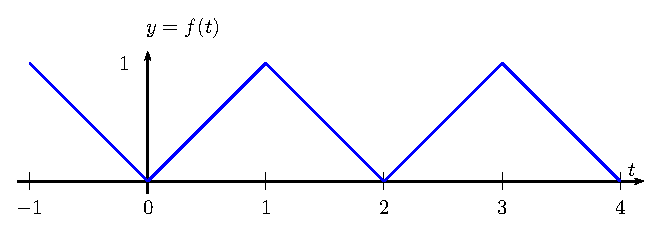
\includegraphics{cap_series/pics/figura_1}
\end{center}
Observamos que essa é uma função par, ou seja, $f(t)=f(-t)$. A fim de explorar essa simetria, utilizaremos as fórmulas (\ref{coef}) envolvendo integrais simétricas, isto é,
  \begin{eqnarray*}
   a_0&=& \frac{2}{T}\int_{-T/2}^{T/2} f(t)dt,\\
   a_n&=&  \frac{2}{T}\int_{-T/2}^{T/2} f(t)\cos(w_nt)dt,\\
   b_n&=&\frac{2}{T}\int_{-T/2}^{T/2} f(t)\sen(w_nt)dt,
  \end{eqnarray*}
onde $T=2$ e $w_n=\frac{2\pi n}{T}=\pi n$. Logo,
  \begin{equation*}
   a_0= \int_{-1}^{1} |t| dt=2\int_{0}^{1} t dt=2\left[\frac{t^2}{2}\right]_0^1=1,
	\end{equation*}
	\begin{eqnarray*}
   a_n=  \int_{-1}^{1} |t|\cos(\pi n t)dt&=&2 \int_{0}^{1} t\cos(\pi n t)dt\\&=&2\left[\frac{t\sen(\pi n t)}{\pi n}\right]_0^1-2\int_0^1\frac{\sen(\pi n t)}{\pi n}dt\\
	&=&2\left[\frac{t\sen(\pi n t)}{\pi n}+\frac{\cos(\pi n t)}{\pi^2 n^2}\right]_0^1=2\frac{(-1)^n-1}{\pi^2n^2},
	 \end{eqnarray*}
	\begin{eqnarray*}
   b_n&=&\int_{-1}^{1} |t|\sen(\pi n t)dt=0.
  \end{eqnarray*}
onde se usou que $|t|$, $|t|\cos(\pi n t)$ são funções pares em $t$ e $|t|\sen(\pi n t)$ é ímpar em $t$. Assim, temos
\begin{equation}
f(t)=\frac{1}{2}-\frac{4}{\pi^2}\left(\cos(\pi t)+\frac{1}{3^2}\cos(3\pi t)+\frac{1}{5^2}\cos(5\pi t) + \cdots\right).
\end{equation}
Observe que, quando $t=0$, obtemos como subproduto da série de Fourier da $f(t)$ a soma da seguinte série numérica:
\begin{equation}\label{serie_inv_impar}
1+\frac{1}{3^2}+\frac{1}{5^2}+\cdots=\frac{\pi^2}{8}.
\end{equation}
A figura \ref{fig_conv_triangular} apresenta os gráficos da série que representa a função $f(t)$ calculada com a séria truncada com um termo, com dois termos e com três termos.
\begin{figure}[!ht]
\begin{center}
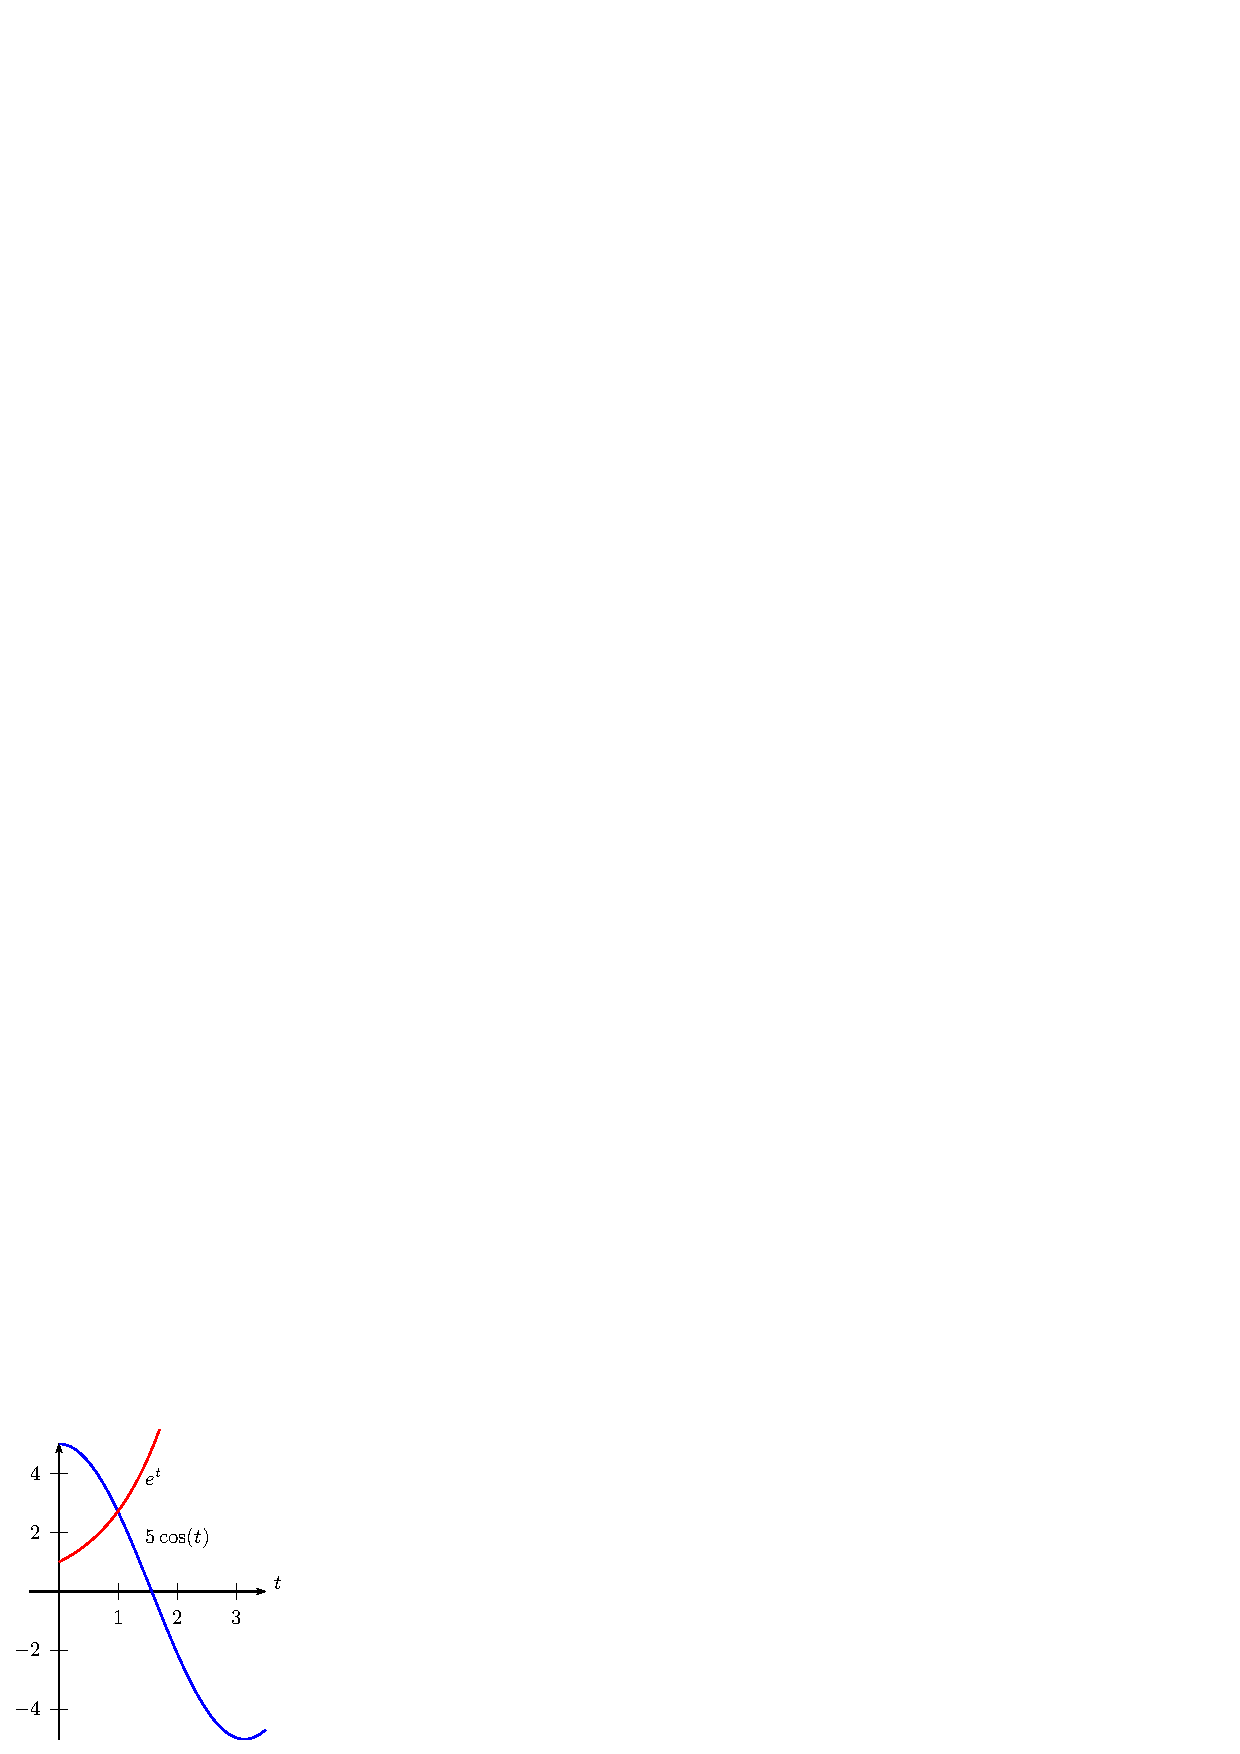
\includegraphics{cap_series/pics/figura_2}\end{center}
\caption{\label{fig_conv_triangular}Gráficos de $f_0(t)=\frac{1}{2}$ (azul), $f_1(t)=\frac{1}{2}-\frac{4}{\pi^2}\cos(\pi t)$ (verde) e $f_2(t)=\frac{1}{2}-\frac{4}{\pi^2}\left(\cos(\pi t)+\frac{1}{3^2}\cos(3\pi t)\right)$ (vermelho).}
\end{figure}
\end{ex}
\begin{ex}\label{ex_quadrada} Seja $g(t)$ uma função dada por
\begin{eqnarray*}
g(t)&=&-1, \ \ -1< t<0,\\
g(t)&=&0, \ \ t=0\ \hbox{ou}\ t=1,\\
g(t)&=&1, \ \ 0< t<1,\\
g(t+2)&=&g(t),\ \ \forall t\in\mathbb{R}.
\end{eqnarray*}
Essa função é suave por partes e contínua em todos os pontos exceto por saltos nos inteiros, onde a função vale a média aritmética dos limites laterais. Portanto se aplica o teorema \ref{teo_Dirichlet}.
\begin{figure}[!ht]
\begin{center}
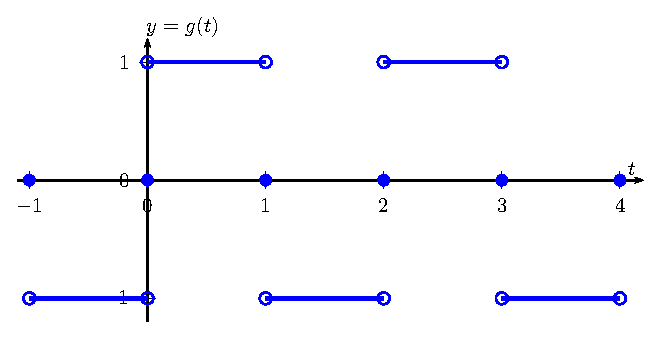
\includegraphics{cap_series/pics/figura_3}\end{center}
\end{figure}
Observamos que essa é uma função ímpar, ou seja, $f(t)=-f(-t)$. Novamente, utilizaremos as fórmulas (\ref{coef}) envolvendo integrais simétricas:
  \begin{eqnarray*}
   a_0 &=& \int_{-1}^{1} g(t) dt=0,\\
	a_n &=&  \int_{-1}^{1} g(t)\cos(\pi n t)dt=0\\
   b_n &=& \int_{-1}^{1} g(t)\sen(\pi n t)dt\\
       &=& 2\int_{0}^{1} g(t)\sen(\pi n t)dt\\
       &=&2\int_{0}^{1} \sen(\pi n t)dt\\
	&=&\frac{2}{\pi n}\left[-\cos(\pi n t)\right]_0^1\\
   &=& 2\frac{1-(-1)^n}{\pi n}.
  \end{eqnarray*}
Logo,
\begin{equation}
g(t)=\frac{4}{\pi}\left(\sen(\pi t)+\frac{1}{3}\sen(3\pi t)+\frac{1}{5}\sen(5\pi t)+\cdots\right).
\end{equation}
A figura \ref{fig_conv_quadrangular} apresenta os gráficos da série que representa a função $g(t)$ com um termo, dois termos, três termos e quatro termos.
\begin{figure}[!ht]
\begin{center}
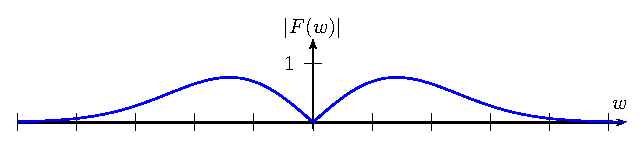
\includegraphics{cap_series/pics/figura_4}\end{center}
\caption{\label{fig_conv_quadrangular}Gráficos de $g_0(t)=\frac{4}{\pi}\sen(\pi t)$ (azul), $g_1(t)=\frac{4}{\pi}\left(\sen(\pi t)+\frac{1}{3}\sen(3\pi t)\right)$ (verde), $g_2(t)=g(t)=\frac{4}{\pi}\left(\sen(\pi t)+\frac{1}{3}\sen(3\pi t)+\frac{1}{5}\sen(5\pi t)\right)$ (vermelho) e $g_3(t)=g(t)=\frac{4}{\pi}\left(\sen(\pi t)+\frac{1}{3}\sen(3\pi t)+\frac{1}{5}\sen(5\pi t)+\frac{1}{7}\sen(7\pi t)\right)$ (preto).}
\end{figure}
\end{ex}
\begin{ex} Seja $h(t)$ uma função dada por
\begin{eqnarray*}
f(t)&=&t, \ \ 0<t<1\\
f(t)&=&\frac{1}{2}, \ \ t=1\\
f(t+1)&=&f(t),\ \ \forall t\in\mathbb{R}.
\end{eqnarray*}
Essa função é suave por partes e contínua exceto por salto nos inteiros onde $h(t)$ assume o valor médio dos limites laterais. Portanto se aplica o teorema \ref{teo_Dirichlet}.
\begin{figure}[!ht]
\begin{center}
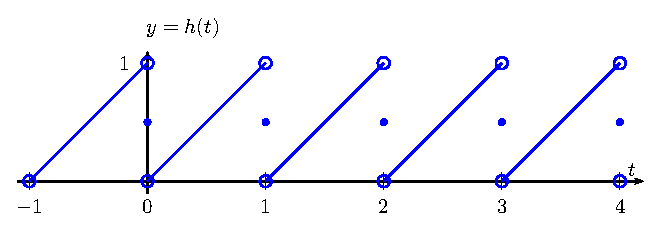
\includegraphics{cap_series/pics/figura_5}\end{center}
\end{figure}
Utilizaremos as fórmulas (\ref{coef}) envolvendo integrais no intervalo $[0,1]$, isto é,
  \begin{eqnarray*}
   a_0&=& 2\int_{0}^{1} t dt=2\left[\frac{t^2}{2}\right]_0^1=1,\\
	a_n&=&  2\int_{0}^{1} t\cos(2 \pi n t)dt\\
   &=&2\left[\frac{t\sen(2 \pi n t)}{2 \pi n}\right]_0^1-2\int_0^1\frac{\sen(2 \pi n t)}{2 \pi n}dt\\
	&=&2\left[\frac{t\sen(2 \pi n t)}{2 \pi n}+\frac{\cos(2 \pi n t)}{4\pi^2 n^2}\right]_0^1=0m\\
	 b_n&=&  2\int_{0}^{1} t\sen(2 \pi n t)dt\\
    &=&2\left[-\frac{t\cos(2 \pi n t)}{2 \pi n}\right]_0^1+2\int_0^1\frac{\cos(2 \pi n t)}{2 \pi n}dt\\
	&=&2\left[-\frac{t\cos(2 \pi n t)}{2 \pi n}+\frac{\sen(2 \pi n t)}{4\pi^2 n^2}\right]_0^1=-\frac{1}{\pi n}.
	 \end{eqnarray*}
Logo,
\begin{equation}
h(t)=\frac{1}{2}-\frac{1}{\pi}\left(\sen(2 \pi t)+\frac{1}{2}\sen(4\pi t)+\frac{1}{3}\sen(6\pi t)+\cdots\right).
\end{equation}
\end{ex}
\begin{obs}{\label{obs_paridade}} Os coeficiente $b_n$ da série de Fourier de uma função par são nulos bem como os coeficiente $a_n$ da série de Fourier de uma função ímpar também o são.
\end{obs}
\begin{ex}Demonstre a observação \ref{obs_paridade}.
\end{ex}
\subsection*{Exercícios}

 \begin{exer}
Considere a função periódica de período $T$ dada na região $(-T/2,T/2)$ por
\begin{equation}f(t)=\left\{
\begin{array}{lc}
0,&-T/2\leq t < -d/2,\\
1,&-d/2\leq t \leq d/2,\\
0,&d/2 < t \leq T/2.
\end{array}
\right.
\end{equation}
onde $d$ é uma constante entre $0$ e $T$.
Estude a paridade desta função. Encontre sua representação em série de Fourier.
\end{exer}
\begin{resp}
\begin{eqnarray*} \frac{a_0}{2}&=&\frac{1}{T}\int_{-T/2}^{T/2}f(t)dt=\frac{1}{T}\int_{-d/2}^{d/2}dt=\frac{d}{T}\\
a_n&=&\frac{2}{T}\int_{-T/2}^{T/2}f(t)\cos(w_nt)dt=\frac{2}{T}\int_{-d/2}^{d/2}\cos(w_nt)dt=\frac{2}{T}\left.\frac{\sen(w_nt)}{w_n}\right|_{-d/2}^{d/2}=\frac{4}{w_nT}\sen(w_nd/2)
\end{eqnarray*}
Como
$w_n=\frac{2\pi n}{T}$, temos $ a_n=\frac{2}{\pi n}\sen\left(\pi n\frac{d}{T}\right)$ e, portanto
\begin{equation}f(t)=\frac{d}{T}+\sum_{n=1}^\infty a_n \cos(w_n t)=\frac{d}{T}+\frac{2}{\pi}\sum_{n=1}^\infty \frac{1}{n}\sen\left(\frac{\pi n d}{T}\right) \cos(w_n t)\end{equation}
\end{resp}
\begin{exer}Considere a função periódica de período $T$ dada para $-T/2<t<T/2$ por
\begin{equation}f(t)=\left\{
\begin{array}{lc}
t,&|t|\leq d/2,\\
0,&d/2<|t|<T/2,\\
\end{array}
\right.
\end{equation}
onde $0<d\leq T$. Calcule sua representação em série de Fourier. Estude o caso particular $d=T$. Dica: $\int u\cos(u)du=\cos(u)+u\sen(u)+C$ e $\int u\sen(u)du=\sen(u)-u\cos(u)+C$.
 \end{exer}
\begin{resp}
 $
b_n=\frac{4}{T}\int_{0}^{d/2}t\sen(w_nt)dt=\frac{T\sen\left(\frac{\pi d n}{T}\right)-dn\pi\cos\left(\frac{\pi d n}{T}\right)}{\pi^2 n^2},~~n\geq 1.
$
e
$
b_n=\frac{T}{\pi n}(-1)^{n+1},~~n\geq 1,~~d=T.
$
\end{resp}
\begin{exer}{\label{Fourier_8}} Trace o gráfico e obtenha a representação em série de Fourier das seguintes funções:
\begin{itemize}
 \item [a)] $f(t)=|\sen(\pi t)|$
 \item [b)] $g(t)=\sum_{n=-\infty}^\infty \delta(t-nT)$ onde $T>0$.
\end{itemize}
\end{exer}
\begin{resp}
\begin{itemize}
 \item [a)] $f(t)=\frac{2}{\pi}- \frac{4}{\pi}\sum_{n=1}^\infty \frac{\cos(2n\pi t)}{4n^2-1}$
\begin{center}
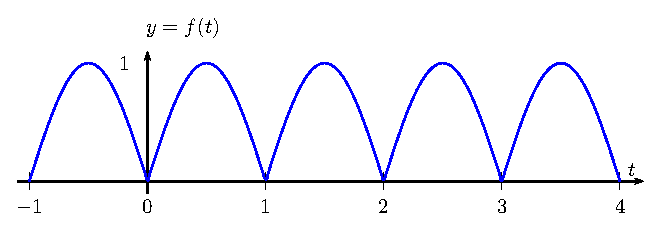
\includegraphics{cap_series/pics/figura_6}\end{center}
 \item [b)] $g(t)=\frac{1}{T}+ \frac{2}{T} \sum_{n=1}^\infty \cos\left(\frac{2\pi n}{T} t\right)$
\begin{center}
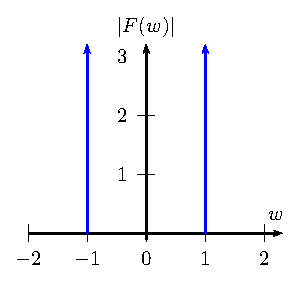
\includegraphics{cap_series/pics/figura_7}\end{center}
 \end{itemize}
\end{resp}
\begin{exer}{\label{Fourier_9}}
 Use o item a do exercício anterior para obter uma representação em Série de Fourier da função \begin{equation}h(t)=|\cos(\pi t)|.\end{equation}
\end{exer}
\begin{resp}
 \begin{eqnarray*}
h(t)&=&f\left(\frac{1}{2}-t\right)=\frac{2}{\pi}- \frac{4}{\pi}\sum_{n=1}^\infty \frac{\cos\left(n\pi-2n\pi t\right)}{4n^2-1}=\frac{2}{\pi}- \frac{4}{\pi}\sum_{n=1}^\infty(-1)^n \frac{\cos\left(2n\pi t\right)}{4n^2-1}
 \end{eqnarray*}
\end{resp}
\begin{exer}Calcule a soma da série:
   \begin{equation}f(t)=\sum_{n=0}^\infty b^{n}\sen(nt),\end{equation}
   onde $0<b<1$ e mostre que:
   \begin{equation}f(t)=\frac{b\sen(t)}{1-2b\cos(t)+b^2}.\end{equation}
   Com base neste resultado, obtenha o valor da integral definida dada por
   \begin{equation}\int_0^{2\pi}\frac{b\sen(t)\sen(kt)}{1-2b\cos(t)+b^2}dt, ~~ k=1,2,3,\ldots.
   \end{equation}
   Dica: Lembre-se de $\sen(x)=\frac{e^{ix}-e^{-ix}}{2i}$ e de $\sum_{x=0}^\infty x^n = \frac{1}{1-x}$ para $|x|<1$.
   \end{exer}
   \begin{resp}
    $\pi b^k$ 
 \end{resp}
   